\chapter {Implementation of Modbus Protocol}
\thispagestyle{empty}
\label{modbus}

\newcommand{\LocMODfig}{\Origin/user-code/modbus/figures}
\newcommand{\LocMODscicode}{\Origin/user-code/modbus/scilab}
\newcommand{\LocMODscibrief}[1]{{\tt \seqsplit{%
        Origin/user-code/modbus/scilab}}, see \fnrefp{fn:file-loc}}
\newcommand{\LocMODardcode}{\Origin/user-code/modbus/arduino}
\newcommand{\LocMODardbrief}[1]{{\tt \seqsplit{%
        Origin/user-code/modbus/arduino}}, see \fnrefp{fn:file-loc}}

%%%%%%%%%%%%python starts
\newcommand{\LocMODpycode}{\Origin/user-code/modbus/python}
\newcommand{\LocMODpybrief}[1]{{\tt \seqsplit{%
        Origin/user-code/modbus/python}}, see \fnrefp{fn:file-loc}}
%%%%%%%%%%%%python ends

%%%%julia starts

\newcommand{\LocMODjuliacode}{\Origin/user-code/modbus/julia}
\newcommand{\LocMODjuliabrief}[1]{{\tt \seqsplit{%
        Origin/user-code/modbus/julia}}, see \fnrefp{fn:file-loc}}

%%%%julia ends


%%%%OpenModelica starts

\newcommand{\LocMODOpenModelicacode}{\Origin/user-code/modbus/OpenModelica}
\newcommand{\LocMODOpenModelicabrief}[1]{{\tt \seqsplit{%
        Origin/user-code/modbus/OpenModelica}}, see \fnrefp{fn:file-loc}}

%%%%OpenModelica ends

In the previous chapters, we have discussed the programs to experiment with the sensors and actuators that come with the Shield, a DC motor, and a servomotor. One may categorize these programs as either basic or intermediate. In this chapter, we will learn one of the advanced applications that can be built using the toolbox. Recall the FLOSS discussed in the book, by default, does not have the capability to connect to Arduino. All such add-on functionalities are added to the FLOSS using toolboxes. Beginners might want to skip this chapter in the first reading. This experiment enables interfacing Modbus-based devices with FLOSS-Arduino toolbox. This functionality has a wide number of applications in the industrial sector.


\section{Preliminaries}
Modbus is an open serial communication protocol developed and
published by Modicon in 1979 \cite{modbus} \cite{modbus-paper}. Because of ease of deployment and maintenance, it finds wide applications in industries. The Modbus protocol provides a means to transmit information over serial lines
between several electronic devices to control and monitor
them. The controlling device requests for reading or writing
information and is known as the Modbus master/client. On the other
hand, the device supplying the information is called
Modbus slave/server. All the slaves/servers have a unique id and
address. Typically, there is one master and a maximum of 247 slaves \cite{simplymodbus}. \figref{mod-block} shows a representation of Modbus protocol.

During the communication on a Modbus network, the protocol determines
how the controller gets to know its device address, recognizes the
the message provided and decides the action to be taken, and accordingly
extracts data and information contained in the message. A typical structure of the communication protocol is shown in \figref{mod-master-slave}.  The data is
sent as a series of zeros and ones, \ie\ bits wherein zeros are sent
as positive voltages and ones as negative.

Different versions of Modbus protocol exist on serial lines, namely
Modbus RTU, ASCII, and TCP \cite{simplymodbus}.
The energy meter used in this chapter
supports the Modbus RTU protocol. In Modbus RTU, the data is coded in
binary and requires only one communication byte. This is ideal for use
over RS232 or RS485 networks at baud rates between 1200 and 115K.

\begin{figure}
  \centering
  %\subfloat[Block diagram representation of the Protocol]{
  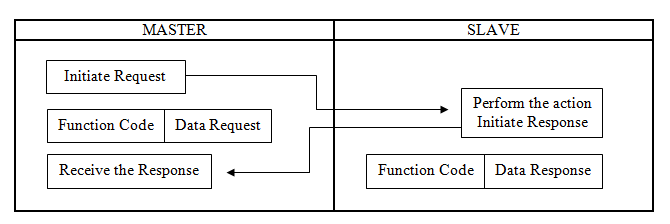
\includegraphics[width=\hgfig]{\LocMODfig/fig1.png}
  \caption{Block diagram representation of the Protocol}
  \label{mod-block}
\end{figure}


\begin{figure}
  \centering
  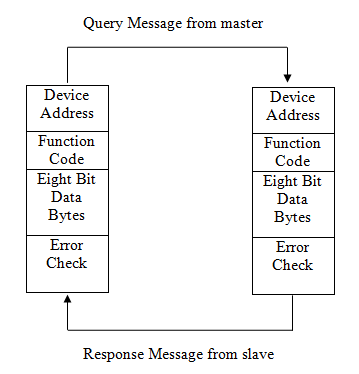
\includegraphics[width=\smfig]{\LocMODfig/fig2.png}
  \caption{Cycle of query-response between master and slave}
  \label{mod-master-slave}
\end{figure}

RS485 is one of the most widely used bus standards for industrial
applications. It uses differential communication lines to communicate
over long distances and requires a dedicated pair of signal lines, say
A and B, to exchange information. Here, the voltage on one line equals
to the inverse of the voltage on the other line. In other words, the
output is 1, if A - B \textgreater $\;$ 200mV, and 0, if B - A \textgreater $\;$
200mV. \figref{rs-485} shows the pins available on a typical RS485 module. As shown in \figref{rs-485}, there are four pins on each side of the module. \tabref{tab:rs-485-pins} summarizes the usage of these pins.

\begin{table}
  \centering
  \caption{Pins available on RS485 and their usage}
  \label{tab:rs-485-pins}
  \begin{tabular}{lc}\hline
    Pin name & Usage                        \\ \hline
    Vcc      & 5V                           \\
    B        & Inverting receiver input     \\
    A        & Non-inverting receiver input \\
    GND      & Ground (0V)                  \\
    RO       & Receiver output              \\
    RE       & Receiver enable              \\
    DE       & Data enable                  \\
    DI       & Data input                   \\
    \hline
  \end{tabular}
\end{table}


%\begin{center}
%\framebox(175,30){%
%   \parbox{170\unitlength}{R0 outputs 1, if A-B\textgreater200mV\\ R0 outputs 0, if B-A\textgreater200mV}%
%}
%\end{center}

%\begin{align*}
%R0 outputs 1, if A-B\textgreater200mV\\
%R0 outputs 0, if B-A\textgreater200mV
%\end{align*}


\begin{figure}
  \centering
  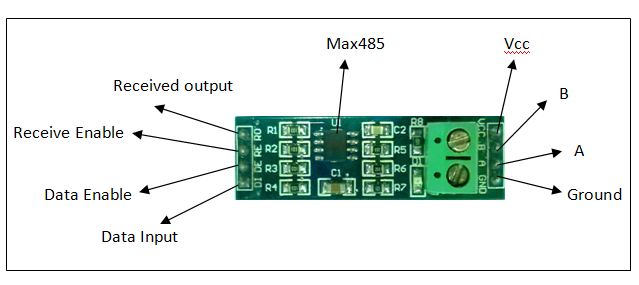
\includegraphics[width=\hgfig]{\LocMODfig/fig3.png}
  \caption{Pins in RS485 module}
  \label{rs-485}
\end{figure}

\subsection{Energy meter}
\label{sec:energy-meter}
An energy meter is a device that measures the amount of electricity consumed
by the load. This book makes use of the EM6400 series energy meter. It is a
multifunction digital power meter by Schneider Electric. It
reads various parameters such as phase voltage, current, active power,
reactive power, power factor, etc. Before using the meter, one has to
program system configuration, PT, CT ratios, communication parameters
through front panel keys. The reason behind using this energy meter is
the fact that it supports the Modbus RTU protocol for communication.

Multiple operations can be performed with devices supporting Modbus.
Every operation has its own fixed function code (coil status - 01,
input status - 02, holding registers - 03, input registers - 04, etc.),
which is independent of devices. The function code tells the slave which
table to access and whether to read from or write to the table.
All the parameter values are stored in the output holding registers.
Different holding registers hold the values of different parameters.
\tabref{tab:modbus-fun-codes} summarizes the various operations which
Modbus RTU supports. One can locate the addresses of individual parameters
in the user manual for EM6400. \tabref{tab:params-addr} provides the addresses
for three individual parameters, which will be accessed in this chapter.


\begin{table}
  \centering
  \caption{Operations supported by Modbus RTU}
  \label{tab:modbus-fun-codes}
  \begin{tabular}{llp{3cm}}\hline
    Function Code & Action         & Table Name                      \\  \hline
    01 (01 hex)   & Read           & Discrete Output Coils           \\
    05 (05 hex)   & Write single   & Discrete Output Coil            \\
    15 (0F hex)   & Write multiple & Discrete Output Coils           \\
    02 (02 hex)   & Read           & Discrete Input Contacts         \\
    04 (04 hex)   & Read           & Analog Input Registers          \\
    03 (03 hex)   & Read           & Analog Output Holding Registers \\
    06 (06 hex)   & Write single   & Analog Output Holding Register  \\
    16 (10 hex)   & Write multiple & Analog Output Holding Registers \\
    \hline
  \end{tabular}
\end{table}


\begin{table}
  \centering
  \caption{Individual parameter address in EM6400}
  \label{tab:params-addr}
  \begin{tabular}{llc}\hline
    Parameter & Description                & Address \\  \hline
    V1        & Voltage phase 1 to neutral & 3927    \\
    A1        & Current, phase 1           & 3929    \\
    W1        & Active power, phase 1      & 3919    \\
    \hline
  \end{tabular}
\end{table}


% \begin{center}
% \begin{tabular}{ll}
% Current (phase 1): & 3929 \\
% Voltage (phase 1): & 3927 \\
% Active power (phase 1): & 3919
% \end{tabular}
% \end{center}

% Values in every register are in little endian format (1st
% register contains LSB and next register contains MSB). In our case,
% energy meter is a slave. 
% As discussed before, slave addresses can be set between 1 and 247. 

In Modbus protocol, the master needs to send a request packet (referred as RQ hereafter)
to the slave to read any of the slave's parameters. When the
slave receives an RQ, it needs to come up with a response packet
(referred as RP hereafter), which contains the value requested
by the master. In other words, an RQ is a message from the
master to a slave and an RP is a message from the slave back to the
master. We will first explain the structure of an RQ, followed by an example.
An RQ consists of the following fields:
\begin{enumerate}
  \item Slave id: The first byte of every Modbus message is a slave id.
        The master specifies the id of the slave to which the request message
        is addressed. Slaves must specify their own id in every
        response message (RP).
  \item Function code: The second byte of every Modbus message is a
        function code. This code determines the type of operation to be
        performed by the slave. \tabref{tab:modbus-fun-codes} enlists the various
        function codes.
  \item Address of the register: After the above two bytes, RQ specifies the
        data address of the first register requested.
  \item Number of registers: This field denotes the total number of
        registers requested.
  \item CRC bytes: The last two bytes of every Modbus message are CRC
        bytes. CRC stands for Cyclic Redundancy check.  It is added to the
        end of every Modbus message for error detection.
        Every byte in the message is used to calculate the CRC.
        The receiving device also calculates the CRC and compares it to the
        CRC from the sending device. If even one bit in the message is
        received incorrectly, the CRCs will be different, resulting in an error.

        \paragraph{Note:} There are some online tools \cite{online-crc} by which one can calculate
        the CRC bytes. However, one should note that the calculated CRC bytes
        should be mentioned in little-endian format, which means that
        the first register contains the least significant bit (LSB) and the
        next register contains the most significant bit (MSB).
\end{enumerate}

Let us say, we want to access V1 (Voltage phase 1 to neutral) in the
energy meter. From \tabref{tab:params-addr}, it may be noted that the address of V1 is 3927. The size of each Modbus register is 16 bits and all EM6400 readings
are of 32 bits. So, each reading occupies two consecutive Modbus
registers. Thus, we need to access two consective holding registers
(starting from 3926) to get V1. \tabref{tab:params-rq} summarizes the
values for the various fields in the RQ required to read/access V1.
\begin{table}
  \centering
  \caption{A request packet to access V1 in EM6400}
  \label{tab:params-rq}
  \begin{tabular}{lc}\hline
    Field of the RQ         & Value for reading V1    \\ \hline
    Slave id                & 01                      \\
    Function code           & 03                      \\
    Address of the register & 3926 (hex value = 0F56) \\
    Number of registers     & 02                      \\
    CRC bytes               & 270F                    \\
    \hline
  \end{tabular}
\end{table}
Now, we explain the structure of an RP, followed by an example.
An RP consists of following fields:
\begin{enumerate}
  \item Slave id: In an RP, the slaves must specify their own id.
  \item Function code: Like the RQ, the second byte of RP is the function code.
        This code determines the type of operation to be
        performed by the slave. \tabref{tab:modbus-fun-codes} enlists the various
        function codes.
  \item Number of data bytes to follow: It refers to the total number of bytes
        read. As our RQ has 2 registers each of two bytes, we expect a total of 4 bytes.
  \item Data in the first requested register: It refers to the data stored
        in the first register.
  \item Data in the second requested register: It refers to the data stored
        in the second register.
  \item CRC bytes: As stated earlier, the last two bytes of every Modbus message are CRC
        bytes. Like RQ, the receiving device also calculates the CRC and compares it to the
        CRC from the sending device.
\end{enumerate}
% An example of a request packet is as follows.  Suppose that
% the request is 01 03 0F56 0002 270F.  Its meaning is explained in
% \tabref{tab:request-packet}.
% \begin{table}
%   \centering
%   \caption{Interpretation of a request packet}
%   \label{tab:request-packet}
%   \begin{tabular}{lp{10cm}}
%     01   & Slave address                                                \\
%     03   & Function code to read holding registers                      \\
%     0F56 & Data Address of the first requested register (address for
%     voltage phase1 to neutral) and 
%     (0F56 hex = 3927, +40001 offset = 43928)                            \\
%     0002 & Total number of registers requested for read                 \\
%     270F & CRC (Cyclic Redundancy Check) for error checking (LSB first) \\
%   \end{tabular}
% \end{table}
Let us consider the RP, which we have received as a response to the RQ mentioned
in \tabref{tab:params-rq}. \tabref{tab:params-rp} summarizes the values for the
various fields in this RP.
\begin{table}
  \centering
  \caption{A response packet to access V1 in EM6400}
  \label{tab:params-rp}
  \begin{tabular}{lc}\hline
    Field of the RP                       & Value for reading V1 \\ \hline
    Slave id                              & 01                   \\
    Function code                         & 03                   \\
    Number of data bytes to follow        & 04                   \\
    Data in the first requested register  & 2921                 \\
    Data in the second requested register & 4373                 \\
    CRC bytes                             & D2B0                 \\
    \hline
  \end{tabular}
\end{table}
% The response packet corresponding the above request packet
% is given as 01 03 04 2921 4373 D2B0.  Its meaning is explained in
% \tabref{tab:response-packet}.
% \begin{table}
%   \centering
%   \caption{Interpretation of a response packet}
%   \label{tab:response-packet}.
%   \begin{tabular}{ll}
%     01   & Slave address                           \\
%     03   & Function code to read holding registers \\
%     04   & Total number of bytes read              \\
%     2921 & Data in 1st requested register          \\
%     4373 & Data in 2st requested register          \\
%     D2B0 & CRC for error checking (LSB first)
%   \end{tabular}
% \end{table}
In this RP, we consider the data in the two requested registers to be 43732921
in hexadecimal. The reason behind keeping the data in the second requested register
as the MSB is that the obtained values are being read in little-endian format.
After converting this value to floating point using the
IEEE Standard for Floating-Point Arithmetic (IEEE 754), we obtain the
value as 243.16. Thus, the value of V1 (Voltage phase 1 to neutral) in the
energy meter is found to be 243.16 Volts.

\subsection{Endianness}
Most of the numeric values to be stored in the computer are more than
one byte long. Thus, there arises a question of how to store the
multibyte values on the computer machines where each byte has its own
address \ie\ which byte gets stored at the ``first'' (lower) memory
location and which bytes follow in higher memory locations. For
example, let us picture this. A two-byte integer 0x5E5F is stored on the disk by one machine, with the 0x5E (MSB) stored at the lower memory address and the 0x5F (LSB) stored at a higher memory address.
But there is a different machine that reads this integer by picking 0x5F for the MSB and 0x5E for the LSB, giving 0x5F5E.
Hence, it results in a disagreement on the value of the integer between the two machines. However, there is no so-called ``right''
ordering to store the bytes in the case of multibyte quantities.
Hardware is built to store the bytes in a particular fashion, and as long as compatible hardware reads the bytes in the same fashion, things are
fine. Following are the two major types of storing the bytes:

\begin{enumerate}
  \item Little-endian:
        If the hardware is designed so that the LSB of a multibyte integer is stored ``first''at the lowest memory address, then the hardware is said to be little-endian. In this format, the ''little'' end of the integer gets stored
        first and the next bytes are stored in higher (increasing) memory
        locations.
  \item Big-endian:
        Here, the hardware is designed so that the MSB of a multibyte integer is stored ``first''at the lowest memory address. Thus, the ``big'' end of the integer gets
        stored first and accordingly the next bytes get stored in higher
        (increasing) memory locations.
\end{enumerate}
For example, let us take a four-byte integer 0x436B84A3. Considering
that the read holding registers in Modbus protocol are 16-bits each, the
LSB (or the little end) of this integer is 0x84A3, and the MSB (or the big end)
of this integer is 0x436B. Then, the memory storage patterns
for the integer would be like that shown in \tabref{tab:memory-storage}.
\begin{table}
  \centering
  \caption{Memory storage of a four-byte integer in little-endian and big-endian}
  \label{tab:memory-storage}
  \begin{tabular}{lllc}\hline
    Memory Address & Byte & Little-endian & Big-endian \\ \hline
    3900           & 8A43 & MSB           & LSB        \\
    3901           & 436B & LSB           & MSB        \\
    \hline
  \end{tabular}
\end{table}

% \begin{table}
%   \centering
%   \caption{Hexadecimal to Decimal}
%   \label{tab:ieee-decimal}
%   \begin{tabular}{ |p{3cm}|p{3cm}|p{3cm}|p{3cm}|}

%     \hline
%     \multicolumn{4}{|c|}{Four Bytes Integer Reading from Meter}  \\
%     \hline

%     Memory Address & Memory Address & Little-endian & Big-endian \\ \hline
%     3900           & 8A43           & MSB           & LSB        \\
%     3901           & 436B           & LSB           & MSB        \\ \hline
%   \end{tabular}
% \end{table}

% \begin{table}
%   \centering
%   \caption{Single and Double Precision Representation}
%   \label{tab:single-precision}
%   \begin{tabular}{|l|l|l|l|}
%     \hline
%     Single & Sign (1 bit) & Exponent (8 bit)  & Mantissa (23 bit) \\ \hline 
%     Double & Sign (1 bit) & Exponent (11 bit) & Mantissa (52 bit) \\ \hline
%   \end{tabular}
% \end{table}


To represent the hexadecimal values of the read holding
registers into user friendly decimal (floating point) values, we
follow IEEE 754 standard. Most common standards for representing
floating point numbers are:
\begin{enumerate}
  \item Single precision: In this standard, 32 bits are used to represent a floating-point number. Out of these 32 bits, one bit is for the sign bit, 8 bits for the exponent, and the remaining 23 bits for mantissa.
  \item Double precision: Here, 64 bits are used to represent a floating-point number. Out of these 64 bits, one bit represents the sign bit, 11 bits for the exponent, and the remaining 52 bits for mantissa. As the name indicates, this standard is used where precision matters more.
\end{enumerate}
% Decimal Value = $( - 1) * \text{sign} * 2^{exponent}* \text{Mantissa}$.
% Hence, for 32 bit values, the sign is stored in bit 32. The exponent
% can be calculated from bits 24-31 by subtracting 127. The mantissa is
% stored in bits 1-23. An invisible leading bit (i.e. it is not actually
% stored) with value 1.0 is placed in front, then bit 23 has a value of
% 1/2, bit 22 has value 1/4 etc. As a result, the mantissa has a value
% between 1.0 and 2. At last, the decimal value is calculated using the
% above mentioned equation. 
There are several online converters \cite{ieee-754-conv} which peform the
IEEE 754 floating point conversion. In this chapter, a function has been formulated for this conversion, wherever needed.


\section{Setup for the experiment}
\begin{figure}
  \centering
  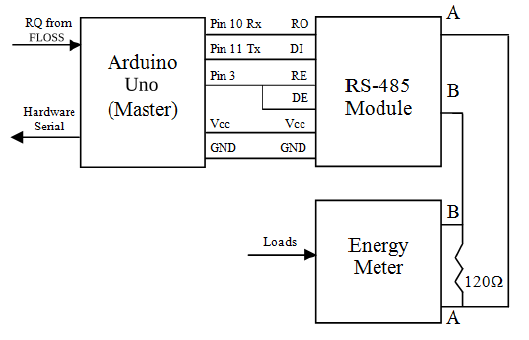
\includegraphics[width=\lgfig]{\LocMODfig/block-diagram.PNG}
  \caption{Block diagram for reading the parameters in energy meter}
  \label{fig:block-diagram}
\end{figure}

\begin{figure}
  \centering
  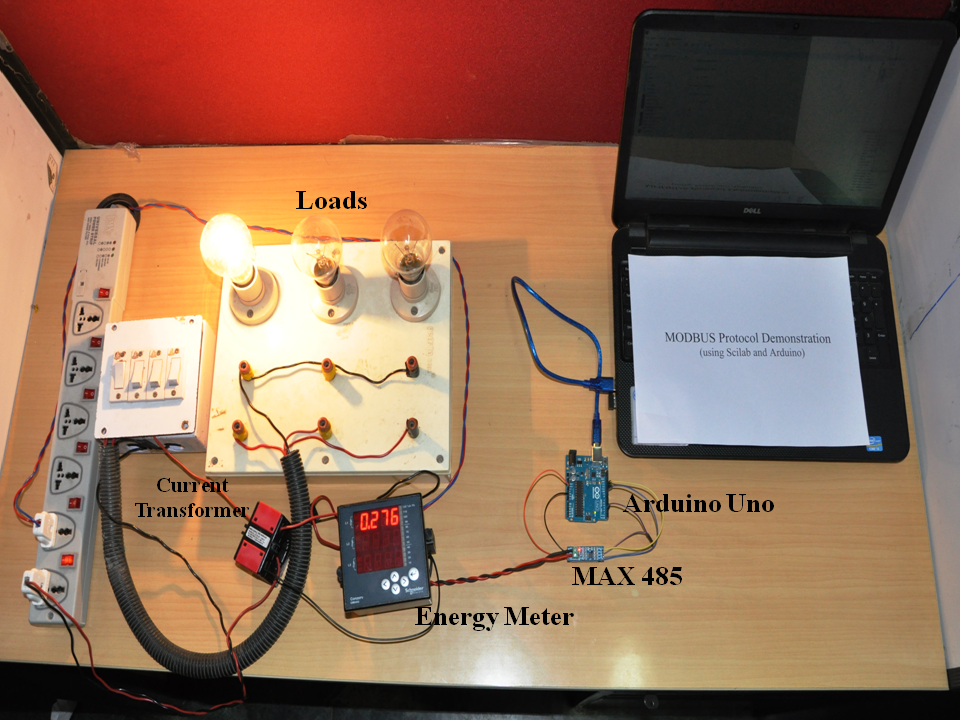
\includegraphics[width=\lgfig]{\LocMODfig/Full-Set-Up.png}
  \caption{Experimental set up for reading energy meter}
  \label{fig:full-set-up}
\end{figure}

This section discusses the setup for configuring
\arduino\ as Modbus master and energy meter as the slave.
The block diagram is shown in \figref{fig:block-diagram} ,
whereas \figref{fig:full-set-up} presents the
actual setup. The following steps discuss the various connections of this setup:
\begin{enumerate}
  \item \arduino\ has only one serial port. It communicates on
        the digital pins 0 and 1 as well as on the computer via USB. Since
        we want serial communication which shouldn't be disturbed by the USB
        port and the Serial Monitor, we use the Software Serial
        library. Using this library, we can assign any digital pins as RX and
        TX and use it for serial communication.
        In this experiment, pin 10 (used as RX) and pin 11 (used as TX) are connected to RO (Receive Out) and DI (Data In) pins of the RS485 module respectively.
  \item DE (Data Enable) and RE (Receive Enable) pins of RS 485 are
        shorted and connected to digital pin 3 of the \arduino\ board.
        This serves as a control pin that will control when to receive and transmit serially.
  \item Vcc and GND of the RS485 module are connected to Vcc and GND of
        the \arduino\ board.
  \item A and B pins of RS485 module are connected to A (Pin 7) and B (Pin 14)
        pins of the energy meter. These two pins of the energy meter are meant for RS485 communication.
  \item A $120k\Omega$ termination resistor is connected between
        pins A and B to avoid reflection losses in the transmission line.
\end{enumerate}

\section{Software required for this experiment}
Apart from FLOSS-Arduino toolbox, the software for this experiment comprises two parts:
\begin{enumerate}
\item  Firmware for \arduino: This firmware is needed to communicate
with the FLOSS (using serial interface), and with RS485 module (using
Software Serial interface). Control logic to enable receive and
transmit modes of MAX485 chip is also present in this firmware. \figref{fig:modbus-firmware} demonstrates the overall implementation of this firmware. The firmware is provided in \secref{sec:firmware-modbus}.

\begin{figure}
  \centering
  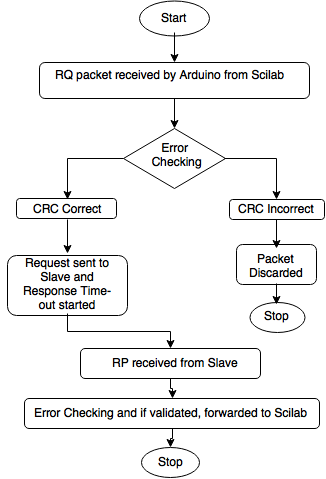
\includegraphics[width=\lgfig]{\LocMODfig/arduino_code_flowchart.png}
  \caption{Flowchart of Arduino firmware}
  \label{fig:modbus-firmware}
\end{figure}

\item FLOSS code: This code requests the parameters in the energy meter
by sending an RQ to \arduino\ from the FLOSS. Then it waits till
an RP is available from the \arduino. After receiving the RP, it extracts
the data from this packet and converts it into IEEE
754 floating-point format. The overall implementation is being
described below:
\begin {enumerate}
  \item Frame an RQ to be sent to the energy meter (slave) in ASCII coded decimal
  format.
  \item Send the RQ serially to \arduino.
  \item Let \arduino\ send the RQ to the energy meter via RS485 module.
  \item Let the energy meter send the RP to \arduino\ via RS485 module.
  \item Read the RP available on \arduino.
  \item Extract the data stored in holding registers from the RP.
  \item Assuming this data to be stored in little-endian format,
  convert this data in floating-point values using IEEE 754 standard.
  \item Display the value in the Console, output window, Command Prompt (on Windows) or Terminal (on Linux), as the case maybe.
\end{enumerate}
\figref{fig:flow-chart} presents the sequence in which the steps mentioned above are executed.
\begin{figure}
  \centering
  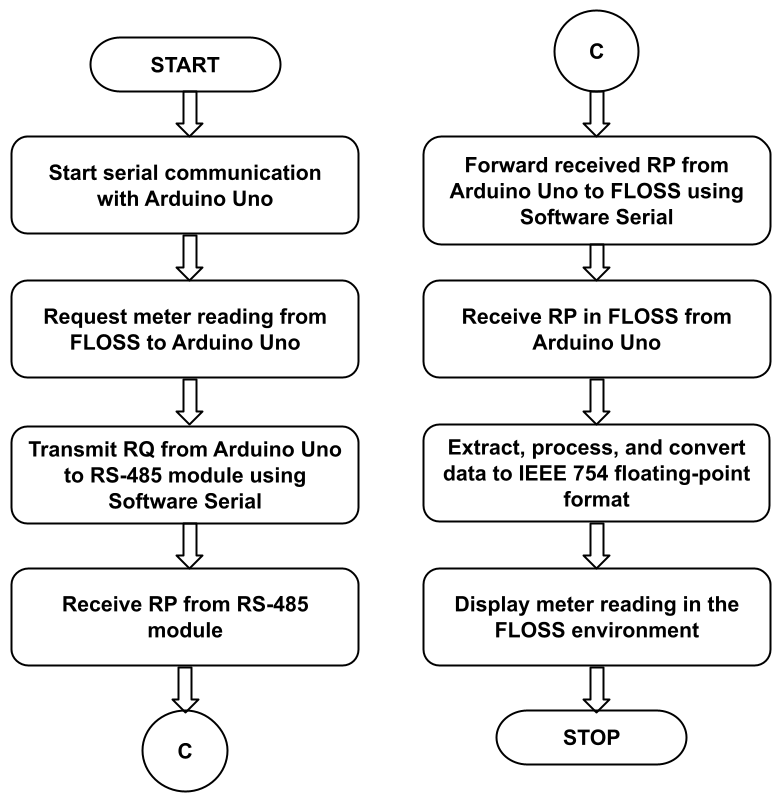
\includegraphics[width=\hgfig]{\LocMODfig/flowchart.png}
  \caption{Flowchart of the steps happening in the FLOSS code}
  \label{fig:flow-chart}
\end{figure}

\end{enumerate}

\subsection{Arduino Firmware}
\label{sec:firmware-modbus}
\addtocontents{ard}{\protect\addvspace{\codclr}}
\begin{ardcode}
  \acaption{First 10 lines of the firmware for Modbus Energy Meter
    experiment}
  {First 10 lines of the firmware for Modbus.  Available at
    \LocMODardbrief{send\_packet.ino}.}
  \label{ard:firmware-modbus}
  \lstinputlisting[firstline=1,lastline=10]
  {\LocMODardcode/send_packet.ino}
\end{ardcode}
